%# -*- coding: utf-8 -*-
%!TEX encoding = UTF-8 Unicode
%!TEX TS-program = xelatex
% vim:ts=4:sw=4
%
% 以上设定默认使用 XeLaTex 编译,并指定 Unicode 编码,供 TeXShop 自动识别

% Author: Yunhui Fu <yhfudev@gmail.com>
% License: Creative Commons (CC BY 4.0)

\section{\cnt{Sparse Coding}{稀疏编码}{}} \label{chp:sparsecoding}

\subsection{\cnt{Sparse Coding}{稀疏编码}{}}

\cnt{Sparse coding is a class of unsupervised methods for learning sets of over-complete bases to represent data efficiently. The aim of sparse coding is to find a set of basis vectors $\mathbf{\phi}_i$ such that we can represent an input vector $\mathbf{x}$ as a linear combination of these basis vectors:}
    {稀疏编码算法是一种无监督学习方法,它用来寻找一组“超完备”基向量来更高效地表示样本数据。稀疏编码算法的目的就是找到一组基向量 $\mathbf{\phi}_i$ ,使得我们能将输入向量 $\mathbf{x}$ 表示为这些基向量的线性组合:}
    {}
\begin{align} \mathbf{x} = \sum_{i=1}^k a_i \mathbf{\phi}_{i} \end{align} 

\cnt{While techniques such as Principal Component Analysis (PCA) allow us to learn a complete set of basis vectors efficiently, we wish to learn an \emph{over-complete} set of basis vectors to represent input vectors $\mathbf{x}\in\mathbb{R}^n$ (i.e. such that $k > n$). The advantage of having an over-complete basis is that our basis vectors are better able to capture structures and patterns inherent in the input data. However, with an over-complete basis, the coefficients ai are no longer uniquely determined by the input vector $\mathbf{x}$. Therefore, in sparse coding, we introduce the additional criterion of \emph{sparsity} to resolve the degeneracy introduced by over-completeness.}
    {虽然形如主成分分析技术(PCA)能使我们方便地找到一组“完备”基向量,但是这里我们想要做的是找到一组“\emph{超完备}”基向量来表示输入向量 $\mathbf{x}\in\mathbb{R}^n$ (也就是说,$k > n$)。超完备基的好处是它们能更有效地找出隐含在输入数据内部的结构与模式。然而,对于超完备基来说,系数 ai 不再由输入向量 $\mathbf{x}$ 唯一确定。因此,在稀疏编码算法中,我们另加了一个评判标准“\emph{稀疏性}”来解决因超完备而导致的退化(degeneracy)问题。}
    {}

\cnt{Here, we define sparsity as having few non-zero components or having few components not close to zero. The requirement that our coefficients $a_i$ be sparse means that given a input vector, we would like as few of our coefficients to be far from zero as possible. The choice of sparsity as a desired characteristic of our representation of the input data can be motivated by the observation that most sensory data such as natural images may be described as the superposition of a small number of atomic elements such as surfaces or edges. Other justifications such as comparisons to the properties of the primary visual cortex have also been advanced.}
    {这里,我们把“稀疏性”定义为:只有很少的几个非零元素或只有很少的几个远大于零的元素。要求系数 $a_i$ 是稀疏的意思就是说:对于一组输入向量,我们只想有尽可能少的几个系数远大于零。选择使用具有稀疏性的分量来表示我们的输入数据是有原因的,因为绝大多数的感官数据,比如自然图像,可以被表示成少量基本元素的叠加,在图像中这些基本元素可以是面或者线。同时,比如与初级视觉皮层的类比过程也因此得到了提升。}
    {}

\cnt{We define the sparse coding cost function on a set of $m$ input vectors as}
    {我们把有 $m$ 个输入向量的稀疏编码代价函数定义为:}
    {}

\begin{align} \text{minimize}_{a^{(j)}_i,\mathbf{\phi}_{i}} \sum_{j=1}^{m} \left|\left| \mathbf{x}^{(j)} - \sum_{i=1}^k a^{(j)}_i \mathbf{\phi}_{i}\right|\right|^{2} + \lambda \sum_{i=1}^{k}S(a^{(j)}_i) \end{align} 
\cnt{where $S(\cdot)$ is a sparsity cost function which penalizes ai for being far from zero. We can interpret the first term of the sparse coding objective as a reconstruction term which tries to force the algorithm to provide a good representation of $\mathbf{x}$ and the second term as a sparsity penalty which forces our representation of $\mathbf{x}$ to be sparse. The constant $\lambda$ is a scaling constant to determine the relative importance of these two contributions.}
    {此处 $S(\cdot)$ 是一个稀疏代价函数,由它来对远大于零的 ai 进行“惩罚”。我们可以把稀疏编码目标函式的第一项解释为一个重构项,这一项迫使稀疏编码算法能为输入向量 $\mathbf{x}$ 提供一个高拟合度的线性表达式,而公式第二项即“稀疏惩罚”项,它使 $\mathbf{x}$ 的表达式变得“稀疏”。常量 $\lambda$ 是一个变换量,由它来控制这两项式子的相对重要性。}
    {}

\cnt{Although the most direct measure of sparsity is the ``$L_0$" norm ($S(a_i) = \mathbf{1}(|a_i|>0)$), it is non-differentiable and difficult to optimize in general. In practice, common choices for the sparsity cost $S(\cdot)$ are the $L_1$ penalty $S(a_i)=\left|a_i\right|_1$ and the log penalty $S(a_i)=\log(1+a_i^2)$.}
    {虽然“稀疏性”的最直接测度标准是 ``$L_0$" 范式($S(a_i) = \mathbf{1}(|a_i|>0)$),但这是不可微的,而且通常很难进行优化。在实际中,稀疏代价函数 $S(\cdot)$ 的普遍选择是 $L_1$ 范式代价函数 $S(a_i)=\left|a_i\right|_1$ 及对数代价函数 $S(a_i)=\log(1+a_i^2)$。}
    {}

\cnt{In addition, it is also possible to make the sparsity penalty arbitrarily small by scaling down $a_i$ and scaling $\mathbf{\phi}_i$ up by some large constant. To prevent this from happening, we will constrain $\left|\left|\mathbf{\phi}\right|\right|^2$ to be less than some constant $C$. The full sparse coding cost function including our constraint on $\mathbf{\phi}$ is}
    {此外,很有可能因为减小 $a_i$ 或增加 $\mathbf{\phi}_i$ 至很大的常量,使得稀疏惩罚变得非常小。为防止此类事件发生,我们将限制 $\left|\left|\mathbf{\phi}\right|\right|^2$ 要小于某常量 $C$。包含了限制条件的稀疏编码代价函数的完整形式如下:}
    {}
$$
\begin{array}{rc} \text{minimize}_{a^{(j)}_i,\mathbf{\phi}_{i}} & \sum_{j=1}^{m} \left|\left| \mathbf{x}^{(j)} - \sum_{i=1}^k a^{(j)}_i \mathbf{\phi}_{i}\right|\right|^{2} + \lambda \sum_{i=1}^{k}S(a^{(j)}_i) \\ \text{subject to} & \left|\left|\mathbf{\phi}_i\right|\right|^2 \leq C, \forall i = 1,...,k \\ \end{array}
$$

\subsubsection{\cnt{Probabilistic Interpretation}{概率解释}{}}
\cnt{[Based on Olshausen and Field 1996]}
    {[基于1996年Olshausen与Field的理论]}
    {}

\cnt{So far, we have considered sparse coding in the context of finding a sparse, over-complete set of basis vectors to span our input space. Alternatively, we may also approach sparse coding from a probabilistic perspective as a generative model.}
    {到目前为止,我们所考虑的稀疏编码,是为了寻找到一个稀疏的、超完备基向量集,来覆盖我们的输入数据空间。现在换一种方式,我们可以从概率的角度出发,将稀疏编码算法当作一种“生成模型”。}
    {}

\cnt{Consider the problem of modelling natural images as the linear superposition of $k$ independent source features $\mathbf{\phi}_i$ with some additive noise $\nu$:}
    {我们将自然图像建模问题看成是一种线性叠加,叠加元素包括 $k$ 个独立的源特征 $\mathbf{\phi}_i$ 以及加性噪声 $\nu$ :}
    {}

\begin{align} \mathbf{x} = \sum_{i=1}^k a_i \mathbf{\phi}_{i} + \nu(\mathbf{x}) \end{align} 

\cnt{Our goal is to find a set of basis feature vectors $\mathbf{\phi}$ such that the distribution of images $P(\mathbf{x}\mid\mathbf{\phi})$ is as close as possible to the empirical distribution of our input data $P^*(\mathbf{x})$. One method of doing so is to minimize the KL divergence between $P^*(\mathbf{x})$ and $P(\mathbf{x}\mid\mathbf{\phi})$ where the KL divergence is defined as:}
    {我们的目标是找到一组特征基向量 $\mathbf{\phi}$,它使得图像的分布函数 $P(\mathbf{x}\mid\mathbf{\phi})$ 尽可能地近似于输入数据的经验分布函数 $P^*(\mathbf{x})$。一种实现方式是,最小化 $P^*(\mathbf{x})$ 与 $P(\mathbf{x}\mid\mathbf{\phi})$ 之间的 KL 散度,此 KL 散度表示如下:}
    {}

\begin{align} D(P^*(\mathbf{x})||P(\mathbf{x}\mid\mathbf{\phi})) = \int P^*(\mathbf{x}) \log \left(\frac{P^*(\mathbf{x})}{P(\mathbf{x}\mid\mathbf{\phi})}\right)d\mathbf{x} \end{align} 

\cnt{Since the empirical distribution $P^*(\mathbf{x})$ is constant across our choice of $\mathbf{\phi}$, this is equivalent to maximizing the log-likelihood of $P(\mathbf{x}\mid\mathbf{\phi})$.}
    {因为无论我们如何选择 $\mathbf{\phi}$,经验分布函数 $P^*(\mathbf{x})$ 都是常量,也就是说我们只需要最大化对数似然函数 $P(\mathbf{x}\mid\mathbf{\phi})$。}
    {}

\cnt{Assuming $\nu$ is Gaussian white noise with variance $\sigma^2$, we have that}
    {假设 $\nu$ 是具有方差 $\sigma^2$ 的高斯白噪音,则有下式:}
    {}
\begin{align} P(\mathbf{x} \mid \mathbf{a}, \mathbf{\phi}) = \frac{1}{Z} \exp\left(- \frac{(\mathbf{x}-\sum^{k}_{i=1} a_i \mathbf{\phi}_{i})^2}{2\sigma^2}\right) \end{align} 

\cnt{In order to determine the distribution $P(\mathbf{x}\mid\mathbf{\phi})$, we also need to specify the prior distribution $P(\mathbf{a})$. Assuming the independence of our source features, we can factorize our prior probability as}
    {为了确定分布 $P(\mathbf{x}\mid\mathbf{\phi})$,我们需要指定先验分布 $P(\mathbf{a})$。假定我们的特征变量是独立的,我们就可以将先验概率分解为:}
    {}
\begin{align} P(\mathbf{a}) = \prod_{i=1}^{k} P(a_i) \end{align} 

\cnt{At this point, we would like to incorporate our sparsity assumption -- the assumption that any single image is likely to be the product of relatively few source features. Therefore, we would like the probability distribution of $a_i$ to be peaked at zero and have high kurtosis. A convenient parameterization of the prior distribution is}
    {此时,我们将“稀疏”假设加入进来——假设任何一幅图像都是由相对较少的一些源特征组合起来的。因此,我们希望 $a_i$ 的概率分布在零值附近是凸起的,而且峰值很高。一个方便的参数化先验分布就是:}
    {}

\begin{align} P(a_i) = \frac{1}{Z}\exp(-\beta S(a_i)) \end{align} 

\cnt{Where $S(a_i)$ is a function determining the shape of the prior distribution.}
    {这里 $S(a_i)$ 是决定先验分布的形状的函数。}
    {}

\cnt{Having defined $P(\mathbf{x} \mid \mathbf{a}$, $\mathbf{\phi})$ and $P(\mathbf{a})$, we can write the probability of the data $\mathbf{x}$ under the model defined by $\mathbf{\phi}$ as}
    {当定义了 $P(\mathbf{x} \mid \mathbf{a}$, $\mathbf{\phi})$ 和 $P(\mathbf{a})$ 后,我们就可以写出在由 $\mathbf{\phi}$ 定义的模型之下的数据 $\mathbf{x}$ 的概率分布:}
    {}

\begin{align} P(\mathbf{x} \mid \mathbf{\phi}) = \int P(\mathbf{x} \mid \mathbf{a}, \mathbf{\phi}) P(\mathbf{a}) d\mathbf{a} \end{align} 

\cnt{and our problem reduces to finding}
    {那么,我们的问题就简化为寻找:}
    {}

\begin{align} \mathbf{\phi}^*=\text{argmax}_{\mathbf{\phi}} < \log(P(\mathbf{x} \mid \mathbf{\phi})) > \end{align} 

\cnt{Where $< \cdot >$ denotes expectation over our input data.}
    {这里 $< \cdot >$ 表示的是输入数据的期望值。}
    {}

\cnt{Unfortunately, the integral over $\mathbf{a}$ to obtain $P(\mathbf{x} \mid \mathbf{\phi})$ is generally intractable. We note though that if the distribution of $P(\mathbf{x} \mid \mathbf{\phi})$ is sufficiently peaked (w.r.t. $\mathbf{a}$), we can approximate its integral with the maximum value of $P(\mathbf{x} \mid \mathbf{\phi})$ and obtain a approximate solution}
    {不幸的是,通过对 $\mathbf{a}$ 的积分计算 $P(\mathbf{x} \mid \mathbf{\phi})$ 通常是难以实现的。虽然如此,我们注意到如果 $P(\mathbf{x} \mid \mathbf{\phi})$ 的分布(对于相应的 $\mathbf{a}$)足够陡峭的话,我们就可以用 $P(\mathbf{x} \mid \mathbf{\phi})$ 的最大值来估算以上积分。估算方法如下:}
    {}

\begin{align} \mathbf{\phi}^{*'}=\text{argmax}_{\mathbf{\phi}} < \max_{\mathbf{a}} \log(P(\mathbf{x} \mid \mathbf{\phi})) > \end{align} 

\cnt{As before, we may increase the estimated probability by scaling down $a_i$ and scaling up $\mathbf{\phi}$ (since $P(a_i)$ peaks about zero) , we therefore impose a norm constraint on our features $\mathbf{\phi}$ to prevent this.}
    {跟之前一样,我们可以通过减小 $a_i$ 或增大 $\mathbf{\phi}$ 来增加概率的估算值(因为 $P(a_i)$ 在零值附近陡升)。因此我们要对特征向量 $\mathbf{\phi}$ 加一个限制以防止这种情况发生。}
    {}

\cnt{Finally, we can recover our original cost function by defining the energy function of this linear generative model}
    {最后,我们可以定义一种线性生成模型的能量函数,从而将原先的代价函数重新表述为:}
    {}
$$
\begin{array}{rl} E\left( \mathbf{x} , \mathbf{a} \mid \mathbf{\phi} \right) & := -\log \left( P(\mathbf{x}\mid \mathbf{\phi},\mathbf{a}\right)P(\mathbf{a})) \\ &= \sum_{j=1}^{m} \left|\left| \mathbf{x}^{(j)} - \sum_{i=1}^k a^{(j)}_i \mathbf{\phi}_{i}\right|\right|^{2} + \lambda \sum_{i=1}^{k}S(a^{(j)}_i) \end{array}
$$
\cnt{where $\lambda = 2\sigma ^2 \beta$ and irrelevant constants have been hidden. Since maximizing the log-likelihood is equivalent to minimizing the energy function, we recover the original optimization problem:}
    {其中 $\lambda = 2\sigma ^2 \beta$,并且关系不大的常量已被隐藏起来。因为最大化对数似然函数等同于最小化能量函数,我们就可以将原先的优化问题重新表述为:}
    {}
\begin{align} \mathbf{\phi}^{*},\mathbf{a}^{*}=\text{argmin}_{\mathbf{\phi},\mathbf{a}} \sum_{j=1}^{m} \left|\left| \mathbf{x}^{(j)} - \sum_{i=1}^k a^{(j)}_i \mathbf{\phi}_{i}\right|\right|^{2} + \lambda \sum_{i=1}^{k}S(a^{(j)}_i) \end{align} 

\cnt{Using a probabilistic approach, it can also be seen that the choices of the $L_1$ penalty $\left|a_i\right|_1$ and the log penalty $\log(1+a_i^2)$ for $S(\cdot)$ correspond to the use of the Laplacian $P(a_i) \propto \exp\left(-\beta|a_i|\right)$ and the Cauchy prior $P(a_i) \propto \frac{\beta}{1+a_i^2}$ respectively.}
    {使用概率理论来分析,我们可以发现,选择 $L_1$ 惩罚和 $\log(1+a_i^2)$ 惩罚作为函数 $S(\cdot)$ ,分别对应于使用了拉普拉斯概率 $P(a_i) \propto \exp\left(-\beta|a_i|\right)$ 和柯西先验概率 $P(a_i) \propto \frac{\beta}{1+a_i^2}$。}
    {}

\subsubsection{\cnt{Learning}{学习算法}{}}

\cnt{Learning a set of basis vectors $\mathbf{\phi}$ using sparse coding consists of performing two separate optimizations, the first being an optimization over coefficients $a_i$ for each training example $\mathbf{x}$ and the second an optimization over basis vectors $\mathbf{\phi}$ across many training examples at once.}
    {使用稀疏编码算法学习基向量集的方法,是由两个独立的优化过程组合起来的。第一个是逐个使用训练样本 $\mathbf{x}$ 来优化系数 $a_i$,第二个是一次性处理多个样本对基向量 $\mathbf{\phi}$ 进行优化。}
    {}

\cnt{Assuming an $L_1$ sparsity penalty, learning $a^{(j)}_i$ reduces to solving a $L_1$ regularized least squares problem which is convex in $a^{(j)}_i$ for which several techniques have been developed (convex optimization software such as CVX can also be used to perform $L_1$ regularized least squares). Assuming a differentiable $S(\cdot)$ such as the log penalty, gradient-based methods such as conjugate gradient methods can also be used.}
    {如果使用 $L_1$ 范式作为稀疏惩罚函数,对 $a^{(j)}_i$ 的学习过程就简化为求解 由 $L_1$ 范式正则化的最小二乘法问题,这个问题函数在域 $a^{(j)}_i$ 内为凸,已经有很多技术方法来解决这个问题(诸如CVX之类的凸优化软件可以用来解决$L_1$正则化的最小二乘法问题)。如果 $S(\cdot)$ 是可微的,比如是对数惩罚函数,则可以采用基于梯度算法的方法,如共轭梯度法。}
    {}

\cnt{Learning a set of basis vectors with a $L_2$ norm constraint also reduces to a least squares problem with quadratic constraints which is convex in $\mathbf{\phi}$. Standard convex optimization software (e.g. CVX) or other iterative methods can be used to solve for $\mathbf{\phi}$ although significantly more efficient methods such as solving the Lagrange dual have also been developed.}
    {用 $L_2$ 范式约束来学习基向量,同样可以简化为一个带有二次约束的最小二乘问题,其问题函数在域 $\mathbf{\phi}$ 内也为凸。标准的凸优化软件(如CVX)或其它迭代方法就可以用来求解 $\mathbf{\phi}$,虽然已经有了更有效的方法,比如求解拉格朗日对偶函数(Lagrange dual)。}
    {}

\cnt{As described above, a significant limitation of sparse coding is that even after a set of basis vectors have been learnt, in order to ``encode" a new data example, optimization must be performed to obtain the required coefficients. This significant ``runtime" cost means that sparse coding is computationally expensive to implement even at test time especially compared to typical feedforward architectures.}
    {根据前面的的描述,稀疏编码是有一个明显的局限性的,这就是即使已经学习得到一组基向量,如果为了对新的数据样本进行“编码”,我们必须再次执行优化过程来得到所需的系数。这个显著的“实时”消耗意味着,即使是在测试中,实现稀疏编码也需要高昂的计算成本,尤其是与典型的前馈结构算法相比。}
    {}


\subsection{\cnt{Sparse Coding: Autoencoder Interpretation}{稀疏编码自编码表达}{}} \label{chp:sparsecodingautoencinterp}

\subsubsection{\cnt{Sparse Coding}{稀疏编码}{}} \label{chp:sparsecodingau}

\cnt{In the sparse autoencoder, we tried to learn a set of weights $W$ (and associated biases $b$) that would give us sparse features $\sigma (Wx + b)$ useful in reconstructing the input $x$.}
    {在稀疏自编码算法中,我们试着学习得到一组权重参数 $W$(以及相应的截距 $b$),通过这些参数可以使我们得到稀疏特征向量 $\sigma (Wx + b)$,这些特征向量对于重构输入样本非常有用。}
    {}
% duplicated figure
\begin{figure}[ht] \centering
  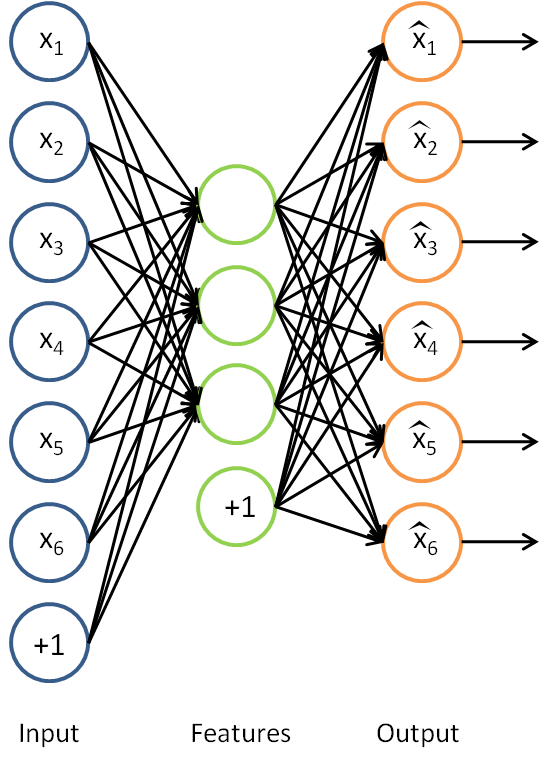
\includegraphics[width=0.4\textwidth]{figures/STL_SparseAE.png}
  %\caption{}\label{fig:step1}
\end{figure}

\cnt{Sparse coding can be seen as a modification of the sparse autoencoder method in which we try to learn the set of features for some data ``directly". Together with an associated basis for transforming the learned features from the feature space to the data space, we can then reconstruct the data from the learned features.}
    {稀疏编码可以看作是稀疏自编码方法的一个变形,该方法试图直接学习数据的特征集。利用与此特征集相应的基向量,将学习得到的特征集从特征空间转换到样本数据空间,这样我们就可以用学习得到的特征集重构样本数据。}
    {}

\cnt{Formally, in sparse coding, we have some data $x$ we would like to learn features on. In particular, we would like to learn $s$, a set of sparse features useful for representing the data, and $A$, a basis for transforming the features from the feature space to the data space. Our objective function is hence:}
    {确切地说,在稀疏编码算法中,有样本数据 $x$ 供我们进行特征学习。特别是,学习一个用于表示样本数据的稀疏特征集 $s$, 和一个将特征集从特征空间转换到样本数据空间的基向量 $A$, 我们可以构建如下目标函数:}
    {}

$$
    J(A, s) = \lVert As - x \rVert_2^2 + \lambda \lVert s \rVert_1 
$$

\cnt{(If you are unfamiliar with the notation, $\lVert x \rVert_k$ refers to the $L_k$ norm of the $x$ which is equal to $\left( \sum{ \left| x_i^k \right|} \right) ^{\frac{1}{k}}.$ The $L_2$ norm is the familiar Euclidean norm, while the $L_1$ norm is the sum of absolute values of the elements of the vector)}
    {($\lVert x \rVert_k$ 是 $x$ 的 $L_k$ 范数,等价于 $\left( \sum{ \left| x_i^k \right|} \right) ^{\frac{1}{k}}$。$L_2$ 范数即大家熟知的欧几里得范数,$L_1$ 范数是向量元素的绝对值之和)}
    {}

\cnt{The first term is the error in reconstructing the data from the features using the basis, and the second term is a sparsity penalty term to encourage the learned features to be sparse.}
    {上式前第一部分是利用基向量将特征集重构为样本数据所产生的误差,第二部分为稀疏性惩罚项(sparsity penalty term),用于保证特征集的稀疏性。}
    {}

\cnt{However, the objective function as it stands is not properly constrained - it is possible to reduce the sparsity cost (the second term) by scaling $A$ by some constant and scaling $s$ by the inverse of the same constant, without changing the error. Hence, we include the additional constraint that that for every column $A_j$ of $A$, $A_j^TA_j \le 1$. Our problem is thus:}
    {但是,如目标函数所示,它的约束性并不强――按常数比例缩放A的同时再按这个常数的倒数缩放 $s$,结果不会改变误差大小,却会减少稀疏代价(表达式第二项)的值。因此,需要为 $A$ 中每项 $A_j$ 增加额外约束 $A_j^TA_j \le 1$。问题变为:}
    {}

$$
    \begin{array}{rcl} {\rm minimize} & \lVert As - x \rVert_2^2 + \lambda \lVert s \rVert_1 \\ {\rm s.t.} & A_j^TA_j \le 1 \; \forall j \\ \end{array} 
$$

\cnt{Unfortunately, the objective function is non-convex, and hence impossible to optimize well using gradient-based methods. However, given $A$, the problem of finding $s$ that minimizes $J(A,s)$ is convex. Similarly, given $s$, the problem of finding $A$ that minimizes $J(A,s)$ is also convex. This suggests that we might try alternately optimizing for $A$ for a fixed $s$, and then optimizing for $s$ given a fixed $A$. It turns out that this works quite well in practice.}
    {遗憾的是,因为目标函数并不是一个凸函数,所以不能用梯度方法解决这个优化问题。但是,在给定 $A$ 的情况下,最小化 $J(A,s)$ 求解 $s$ 是凸的。同理,给定 $s$ 最小化 $J(A,s)$ 求解 $A$ 也是凸的。这表明,可以通过交替固定 $s$ 和 $A$ 分别求解 $A$ 和 $s$。实践表明,这一策略取得的效果非常好。}
    {}

\cnt{However, the form of our problem presents another difficulty - the constraint that $A_j^TA_j \le 1 \; \forall j$ cannot be enforced using simple gradient-based methods. Hence, in practice, this constraint is weakened to a ``weight decay" term designed to keep the entries of $A$ small. This gives us a new objective function:}
    {但是,以上表达式带来了另一个难题:不能用简单的梯度方法来实现约束条件 $A_j^TA_j \le 1 \; \forall j$。因此在实际问题中,此约束条件还不足以成为“权重衰变”(``weight decay")项以保证 $A$ 的每一项值够小。这样我们就得到一个新的目标函数:}
    {}

$$
    J(A, s) = \lVert As - x \rVert_2^2 + \lambda \lVert s \rVert_1 + \gamma \lVert A \rVert_2^2 
$$

\cnt{(note that the third term, $\lVert A \rVert_2^2$ is simply the sum of squares of the entries of $A$, or $\sum_r{\sum_c{A_{rc}^2}})$}
    {(注意上式中第三项, $\lVert A \rVert_2^2$ 等价于 $\sum_r{\sum_c{A_{rc}^2}}$,是 $A$ 各项的平方和)}
    {}

\cnt{This objective function presents one last problem - the $L_1$ norm is not differentiable at 0, and hence poses a problem for gradient-based methods. While the problem can be solved using other non-gradient descent-based methods, we will ``smooth out" the $L_1$ norm using an approximation which will allow us to use gradient descent. To ``smooth out" the $L_1$ norm, we use $\sqrt{x^2 + \epsilon}$ in place of $\left| x \right|$, where $\epsilon$ is a ``smoothing parameter" which can also be interpreted as a sort of ``sparsity parameter" (to see this, observe that when $\epsilon$ is large compared to $x$, the $x + \epsilon$ is dominated by $\epsilon$, and taking the square root yields approximately $\sqrt{\epsilon}$). This ``smoothing" will come in handy later when considering topographic sparse coding below.}
    {这一目标函数带来了最后一个问题,即 $L_1$ 范数在 0 点处不可微影响了梯度方法的应用。尽管可以通过其他非梯度下降方法避开这一问题,但是本文通过使用近似值“平滑” $L_1$ 范数的方法解决此难题。使用 $\sqrt{x^2 + \epsilon}$ 代替 $\left| x \right|$, 对 $L_1$ 范数进行平滑,其中 $\epsilon$ 是“平滑参数”(``smoothing parameter")或者“稀疏参数”(``sparsity parameter") (如果 $\epsilon$ 远大于 $x$, 则 $x + \epsilon$ 的值由 $\epsilon$ 主导,其平方根近似于 $\epsilon$)。在下文提及拓扑稀疏编码时,“平滑”会派上用场。}
    {}

\cnt{Our final objective function is hence:}
    {因此,最终的目标函数是:}
    {}
$$
    J(A, s) = \lVert As - x \rVert_2^2 + \lambda \sqrt{s^2 + \epsilon} + \gamma \lVert A \rVert_2^2 
$$
\cnt{(where $\sqrt{s^2 + \epsilon}$ is shorthand for $\sum_k{\sqrt{s_k^2 + \epsilon}}$)}
    {}
    {}

\cnt{This objective function can then be optimized iteratively, using the following procedure:}
    {该目标函数可以通过以下过程迭代优化:}
    {}

\begin{enumerate}
  \item \cnt{Initialize $A$ randomly}{随机初始化$A$}{}{}
  \item \cnt{Repeat until convergence}{重复以下步骤直至收敛:}{}{}
    \begin{enumerate}
      \item \cnt{Find the $s$ that minimizes $J(A,s)$ for the $A$ found in the previous step}
                {根据上一步给定的 $A$,求解能够最小化 $J(A,s)$ 的 $s$}
                {}

      \item \cnt{Solve for the $A$ that minimizes $J(A,s)$ for the $s$ found in the previous step}
                {根据上一步得到的$s$,求解能够最小化 $J(A,s)$ 的 $A$}
                {}
    \end{enumerate}
\end{enumerate}

\cnt{Observe that with our modified objective function, the objective function $J(A,s)$ given $s$, that is $J(A; s) = \lVert As - x \rVert_2^2 + \gamma \lVert A \rVert_2^2$ (the $L_1$ term in $s$ can be omitted since it is not a function of $A$) is simply a quadratic term in $A$, and hence has an easily derivable analytic solution in $A$. A quick way to derive this solution would be to use matrix calculus - some pages about matrix calculus can be found in the useful links section(\ref{chp:usefullinks}). Unfortunately, the objective function given $A$ does not have a similarly nice analytic solution, so that minimization step will have to be carried out using gradient descent or similar optimization methods.}
    {观察修改后的目标函数 $J(A,s)$,给定 $s$ 的条件下,目标函数可以简化为 $J(A; s) = \lVert As - x \rVert_2^2 + \gamma \lVert A \rVert_2^2$(因为 $s$ 的 $L_1$ 范式不是 $A$ 的函数,所以可以忽略)。简化后的目标函数是一个关于 $A$ 的简单二次项式,因此对 $A$ 求导是很容易的。这种求导的一种快捷方法是矩阵微积分( 相关链接部分列出了跟矩阵演算有关的内容)。遗憾的是,在给定 $A$ 的条件下,目标函数却不具备这样的求导方法,因此目标函数的最小化步骤只能用梯度下降或其他类似的最优化方法。}
    {}

\cnt{In theory, optimizing for this objective function using the iterative method as above should (eventually) yield features (the basis vectors of $A$) similar to those learned using the sparse autoencoder. However, in practice, there are quite a few tricks required for better convergence of the algorithm, and these tricks are described in greater detail in the later section on sparse coding in practice(\ref{chp:practsparsecoding}). Deriving the gradients for the objective function may be slightly tricky as well, and using matrix calculus or using the backpropagation intuition(\ref{chp:derivegradbackpropidea}) can be helpful.}
    {理论上,通过上述迭代方法求解目标函数的最优化问题最终得到的特征集($A$ 的基向量)与通过稀疏自编码学习得到的特征集是差不多的。但是实际上,为了获得更好的算法收敛性需要使用一些小技巧,后面的 稀疏编码实践 稀疏编码实践章节会详细介绍这些技巧。用梯度下降方法求解目标函数也略需技巧,另外使用矩阵演算或 反向传播算法则有助于解决此类问题。}
    {}

\subsubsection{\cnt{Topographic sparse coding}{拓扑稀疏编码}{}} \label{chp:topogsparsecoding}

\cnt{With sparse coding, we can learn a set of features useful for representing the data. However, drawing inspiration from the brain, we would like to learn a set of features that are ``orderly" in some manner. For instance, consider visual features. As suggested earlier, the V1 cortex of the brain contains neurons which detect edges at particular orientations. However, these neurons are also organized into hypercolumns in which adjacent neurons detect edges at similar orientations. One neuron could detect a horizontal edge, its neighbors edges oriented slightly off the horizontal, and moving further along the hypercolumn, the neurons detect edges oriented further off the horizontal.}
    {通过稀疏编码,我们能够得到一组用于表示样本数据的特征集。不过,让我们来找些灵感,我们希望学习得到一组有某种“秩序”的特征集。举个例子,视觉特征,如前面所提到的,大脑皮层 V1 区神经元能够按特定的方向对边缘进行检测,同时,这些神经元(在生理上)被组织成超柱(hypercolumns),在超柱中,相邻神经元以相似的方向对边缘进行检测,一个神经元检测水平边缘,其相邻神经元检测到的边缘就稍微偏离水平方向,沿着超柱,神经元就可以检测到与水平方向相差更大的边缘了。}
    {}

\cnt{Inspired by this example, we would like to learn features which are similarly ``topographically ordered". What does this imply for our learned features? Intuitively, if ``adjacent" features are ``similar", we would expect that if one feature is activated, its neighbors will also be activated to a lesser extent.}
    {受该例子的启发,我们希望学习到的特征也具有这样“拓扑秩序”的性质。这对于我们要学习的特征意味着什么呢?直观的讲,如果“相邻”的特征是“相似”的,就意味着如果某个特征被激活,那么与之相邻的特征也将随之被激活。}
    {}

\cnt{Concretely, suppose we (arbitrarily) organized our features into a square matrix. We would then like adjacent features in the matrix to be similar. The way this is accomplished is to group these adjacent features together in the smoothed L1 penalty, so that instead of say $\sqrt{s_{1,1}^2 + \epsilon}$, we use say $\sqrt{s_{1,1}^2 + s_{1,2}^2 + s_{1,3}^2 + s_{2,1}^2 + s_{2,2}^2 + s_{3,2}^2 + s_{3,1}^2 + s_{3,2}^2 + s_{3,3}^2 + \epsilon}$ instead, if we group in $3 \times 3$ regions. The grouping is usually overlapping, so that the $3 \times 3$ region starting at the 1st row and 1st column is one group, the $3 \times 3$ region starting at the 1st row and 2nd column is another group, and so on. Further, the grouping is also usually done wrapping around, as if the matrix were a torus, so that every feature is counted an equal number of times.}
    {具体而言,假设我们(随意地)将特征组织成一个方阵。我们就希望矩阵中相邻的特征是相似的。实现这一点的方法是将相邻特征按经过平滑的L1范式惩罚进行分组,如果按 $3 \times 3$ 方阵分组,则用 $\sqrt{s_{1,1}^2 + s_{1,2}^2 + s_{1,3}^2 + s_{2,1}^2 + s_{2,2}^2 + s_{3,2}^2 + s_{3,1}^2 + s_{3,2}^2 + s_{3,3}^2 + \epsilon}$ 代替 $\sqrt{s_{1,1}^2 + \epsilon}$, 其分组通常是重合的,因此从第 1 行第 1 列开始的 $3 \times 3$ 区域是一个分组,从第 1 行第 2 列开始的 $3 \times 3$ 区域是另一个分组,以此类推。最终,这样的分组会形成环绕,就好像这个矩阵是个环形曲面,所以每个特征都以同样的次数进行了分组。}
    {}

\cnt{Hence, in place of the smoothed L1 penalty, we use the sum of smoothed L1 penalties over all the groups, so our new objective function is:}
    {于是,将经过平滑的所有分组的 L1 惩罚值之和代替经过平滑的 L1 惩罚值,得到新的目标函数如下:}
    {}
$$
    J(A, s) = \lVert As - x \rVert_2^2 + \lambda \sum_{\text{all groups} g}{\sqrt{ \left( \sum_{\text{all} s \in g}{s^2} \right) + \epsilon}} + \gamma \lVert A \rVert_2^2 
$$

\cnt{In practice, the ``grouping" can be accomplished using a ``grouping matrix" $V$, such that the $r$th row of $V$ indicates which features are grouped in the $r$th group, so $V_{r,c} = 1$ if group $r$ contains feature $c$. Thinking of the grouping as being achieved by a grouping matrix makes the computation of the gradients more intuitive. Using this grouping matrix, the objective function can be rewritten as:}
    {实际上,“分组”可以通过“分组矩阵” $V$ 完成,于是矩阵 $V$ 的第 $r$ 行标识了哪些特征被分到第 $r$ 组中,即如果第 $r$ 组包含特征 $c$ 则 $V_{r,c} = 1$。通过分组矩阵实现分组使得梯度的计算更加直观,使用此分组矩阵,目标函数被重写为:}
    {}

$$
    J(A, s) = \lVert As - x \rVert_2^2 + \lambda \sum{ \sqrt{Vss^T + \epsilon}} + \gamma \lVert A \rVert_2^2 
$$

\cnt{(where $\sum{ \sqrt{Vss^T + \epsilon}}$ is $\sum_r \sum_c D_{r,c}$ if we let $D = \sqrt{Vss^T + \epsilon}$)}
    {(令 $D = \sqrt{Vss^T + \epsilon}$,$\sum{ \sqrt{Vss^T + \epsilon}}$ 等价于 $\sum_r \sum_c D_{r,c}$}
    {}

\cnt{This objective function can be optimized using the iterated method described in the earlier section. Topographic sparse coding will learn features similar to those learned by sparse coding, except that the features will now be ``ordered" in some way.}
    {该目标函数能够使用之前部分提到的迭代方法进行求解。拓扑稀疏编码得到的特征与稀疏编码得到的类似,只是拓扑稀疏编码得到的特征是以某种方式有“秩序”排列的。}
    {}


\subsubsection{\cnt{Sparse coding in practice}{稀疏编码实践}{}} \label{chp:practsparsecoding}

\cnt{As suggested in the earlier sections, while the theory behind sparse coding is quite simple, writing a good implementation that actually works and converges reasonably quickly to good optima requires a bit of finesse.}
    {如上所述,虽然稀疏编码背后的理论十分简单,但是要写出准确无误的实现代码并能快速又恰到好处地收敛到最优值,则需要一定的技巧。}
    {}

\cnt{Recall the simple iterative algorithm proposed earlier:}
    {回顾一下之前提到的简单迭代算法:}
    {}
\begin{enumerate}
  \item \cnt{Initialize $A$ randomly}{随机初始化$A$}{}
  \item \cnt{Repeat until convergence}{重复以下步骤直至收敛到最优值:}{}
    \begin{enumerate}
      \item \cnt{Find the $s$ that minimizes $J(A,s)$ for the $A$ found in the previous step}{根据上一步给定的 $A$,求解能够最小化 $J(A,s)$ 的 $s$}{}
      \item \cnt{Solve for the $A$ that minimizes $J(A,s)$ for the $s$ found in the previous step}{根据上一步得到的$s$,求解能够最小化 $J(A,s)$ 的 $A$}{}
    \end{enumerate}
\end{enumerate}

\cnt{It turns out that running this algorithm out of the box will not produce very good results, if any results are produced at all. There are two main tricks to achieve faster and better convergence:}
    {这样信手拈来地执行这个算法,结果并不会令人满意,即使确实得到了某些结果。以下是两种更快更优化的收敛技巧:}
    {}


\begin{enumerate}
  \item \cnt{Batching examples into ``mini-batches"}{将样本分批为“迷你块”}{}
  \item \cnt{Good initialization of $s$}{良好的$s$初始值}{}
\end{enumerate}

\textbf{\cnt{Batching examples into mini-batches}{将样本分批为“迷你块”}{}}

\cnt{If you try running the simple iterative algorithm on a large dataset of say 10 000 patches at one go, you will find that each iteration takes a long time, and the algorithm may hence take a long time to converge. To increase the rate of convergence, you can instead run the algorithm on mini-batches instead. To do this, instead of running the algorithm on all 10 000 patches, in each iteration, select a mini-batch - a (different) random subset of say 2000 patches from the 10 000 patches - and run the algorithm on that mini-batch for the iteration instead. This accomplishes two things - firstly, it speeds up each iteration, since now each iteration is operating on 2000 rather than 10 000 patches; secondly, and more importantly, it increases the rate of convergence (TODO: explain why).}
    {如果你一次性在大规模数据集(比如,有10000 个patch)上执行简单的迭代算法,你会发现每次迭代都要花很长时间,也因此这算法要花好长时间才能达到收敛结果。为了提高收敛速度,可以选择在迷你块上运行该算法。每次迭代的时候,不是在所有的 10000 个 patchs 上执行该算法,而是使用迷你块,即从 10000 个 patch 中随机选出 2000 个 patch,再在这个迷你块上执行这个算法。这样就可以做到一石二鸟――第一,提高了每次迭代的速度,因为现在每次迭代只在 2000 个 patch 上执行而不是 10000个;第二,也是更重要的,它提高了收敛的速度(原因见TODO)。}
    {}


\textbf{\cnt{Good initialization of $s$}{良好的$s$初始值}{}}

\cnt{Another important trick in obtaining faster and better convergence is good initialization of the feature matrix $s$ before using gradient descent (or other methods) to optimize for the objective function for s given $A$. In practice, initializing $s$ randomly at each iteration can result in poor convergence unless a good optima is found for $s$ before moving on to optimize for $A$. A better way to initialize $s$ is the following:}
    {另一个能获得更快速更优化收敛的重要技巧是:在给定 $A$ 的条件下,根据目标函数使用梯度下降(或其他方法)求解 $s$ 之前找到良好的特征矩阵 $s$ 的初始值。实际上,除非在优化 $A$ 的最优值前已找到一个最佳矩阵 $s$,不然每次迭代过程中随机初始化 $s$ 值会导致很差的收敛效果。下面给出一个初始化 $s$ 的较好方法:}
    {}
\begin{enumerate}
  \item \cnt{Set $s \leftarrow W^Tx$ (where $x$ is the matrix of patches in the mini-batch)}
    {令 $s \leftarrow W^Tx$ ($x$ 是迷你块中patches的矩阵表示)}
    {}

  \item \cnt{For each feature in $s$ (i.e. each column of $s$), divide the feature by the norm of the corresponding basis vector in $A$. That is, if $s_{r,c}$ is the $r$th feature for the $c$th example, and $A_c$ is the $c$th basis vector in $A$, then set $s_{r, c} \leftarrow \frac{ s_{r, c}} { \lVert A_c \rVert}$.}
    {s中的每个特征($s$的每一列),除以其在$A$中对应基向量的范数。即,如果$s_{r,c}$表示第$c$个样本的第$r$个特征,则$A_c$表示$A$中的第$c$个基向量,则令 $s_{r, c} \leftarrow \frac{ s_{r, c}} { \lVert A_c \rVert}$.}
    {}
\end{enumerate}

\cnt{Very roughly and informally speaking, this initialization helps because the first step is an attempt to find a good $s$ such that $Ws \approx x$, and the second step ``normalizes" $s$ in an attempt to keep the sparsity penalty small. It turns out that initializing $s$ using only one but not both steps results in poor performance in practice. (TODO: a better explanation for why this initialization helps?)}
    {无疑,这样的初始化有助于算法的改进,因为上述的第一步希望找到满足 $Ws \approx x$ 的矩阵 $s$;第二步对 $s$ 作规范化处理是为了保持较小的稀疏惩罚值。这也表明,只采用上述步骤的某一步而不是两步对 $s$ 做初始化处理将严重影响算法性能。(TODO: 此链接将会对为什么这样的初始化能改进算法作出更详细的解释)}
    {}


\textbf{\cnt{The practical algorithm}{可运行算法}{}}

\cnt{With the above two tricks, the algorithm for sparse coding then becomes:}
    {有了以上两种技巧,稀疏编码算法修改如下:}
    {}
\begin{enumerate}
  \item \cnt{Initialize $A$ randomly}{随机初始化$A$}{}
  \item \cnt{Repeat until convergence}{重复以下步骤直至收敛}{}
    \begin{enumerate}
      \item \cnt{Select a random mini-batch of 2000 patches}{随机选取一个有2000个patches的迷你块}{}
      \item \cnt{Initialize $s$ as described above}{如上所述,初始化s}{}
      \item \cnt{Find the $s$ that minimizes $J(A,s)$ for the $A$ found in the previous step}{根据上一步给定的$A$,求解能够最小化$J(A,s)$的$s$}{}
      \item \cnt{Solve for the $A$ that minimizes $J(A,s)$ for the $s$ found in the previous step}{根据上一步得到的$s$,求解能够最小化$J(A,s)$的$A$}{}
    \end{enumerate}
\end{enumerate}

\cnt{With this method, you should be able to reach a good local optima relatively quickly.}
    {通过上述方法,可以相对快速的得到局部最优解。}
    {}



\subsection{\cnt{Exercise:Sparse Coding}{}{}}

\cnt{In this exercise, you will implement sparse coding(\ref{chp:sparsecodingae}) and topographic sparse coding(\ref{chp:topogsparsecoding}) on black-and-white natural images.}
    {}
    {}

\cnt{In the file \href{http://ufldl.stanford.edu/wiki/resources/sparse_coding_exercise.zip}{sparse\_coding\_exercise.zip} we have provided some starter code. You should write your code at the places indicated ``YOUR CODE HERE" in the files.}
    {}
    {}

\cnt{For this exercise, you will need to modify sparseCodingWeightCost.m, sparseCodingFeatureCost.m and sparseCodingExercise.m.}
    {}
    {}

\subsubsection{\cnt{Dependencies}{}{}}
    {}
    {}

\cnt{You will need:}
    {}
    {}
\begin{itemize}
  \item \cnt{\texttt{computeNumericalGradient.m} from Exercise:Sparse Autoencoder (\ref{chp:execsparseautoenc})}
    {}
    {}
  \item \cnt{\texttt{display\_network.m} from Exercise:Sparse Autoencoder (\ref{chp:execsparseautoenc})}
    {}
    {}
\end{itemize}

\emph{
\cnt{If you have not completed the exercise listed above, we strongly suggest you complete it first.}
    {}
    {}
}

\subsubsection{\cnt{Step 0: Initialization}{}{}}

\cnt{In this step, we initialize some parameters used for the exercise.}
    {}
    {}

\subsubsection{\cnt{Step 1: Sample patches}{}{}}

\cnt{In this step, we sample some patches from the \texttt{IMAGES.mat} dataset comprising 10 black-and-white pre-whitened natural images.}
    {}
    {}

\subsubsection{\cnt{Step 2: Implement and check sparse coding cost functions}{}{}}

\cnt{In this step, you should implement the two sparse coding cost functions:}
    {}
    {}
\begin{enumerate}
  \item \cnt{\texttt{sparseCodingWeightCost} in \texttt{sparseCodingWeightCost.m}, which is used for optimizing the weight cost given the features}
    {}
    {}
  \item \cnt{\texttt{sparseCodingFeatureCost} in \texttt{sparseCodingFeatureCost.m}, which is used for optimizing the feature cost given the weights}
    {}
    {}
\end{enumerate}

\cnt{Each of these functions should compute the appropriate cost and gradient. You may wish to implement the non-topographic version of sparseCodingFeatureCost first, ignoring the grouping matrix and assuming that none of the features are grouped. You can then extend this to the topographic version later. Alternatively, you may implement the topographic version directly - using the non-topographic version will then involve setting the grouping matrix to the identity matrix.}
    {}
    {}

\cnt{Once you have implemented these functions, you should check the gradients numerically.}
    {}
    {}

\cnt{\emph{Implementation tip} - gradient checking the feature cost. One particular point to note is that when checking the gradient for the feature cost, \texttt{epsilon} should be set to a larger value, for instance \texttt{1e-2} (as has been done for you in the checking code provided), to ensure that checking the gradient numerically makes sense. This is necessary because as \texttt{epsilon} becomes smaller, the function \texttt{sqrt(x + epsilon)} becomes ``sharper" and more ``pointed", making the numerical gradient computed near 0 less and less accurate. To see this, consider what would happen if the numerical gradient was computed by using a point with x less than 0 and a point with x greater than 0 - the computed numerical slope would be wildly inaccurate.}
    {}
    {}

\subsubsection{\cnt{Step 3: Iterative optimization}{}{}}

\cnt{In this step, you will iteratively optimize for the weights and features to learn a basis for the data, as described in the section on sparse coding(\ref{chp:sparsecodingautoencinterp}). Mini-batching and initialization of the features s has already been done for you. However, you need to still need to fill in the analytic solution to the the optimization problem with respect to the weight matrix, given the feature matrix.}
    {}
    {}

\cnt{Once that is done, you should check that your solution is correct using the given checking code, which checks that the gradient at the point determined by your analytic solution is close to 0. Once your solution has been verified, comment out the checking code, and run the iterative optimization code. 200 iterations should take less than 45 minutes to run, and by 100 iterations you should be able to see bases that look like edges, similar to those you learned in the sparse autoencoder exercise(\ref{chp:execsparseautoenc}).}
    {}
    {}

\cnt{For the non-topographic case, these features will not be ``ordered", and will look something like the following:}
    {}
    {}
\begin{figure}[ht] \centering
  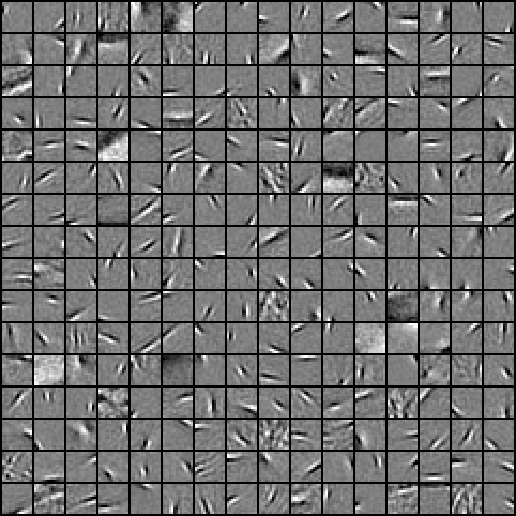
\includegraphics[width=0.4\textwidth]{figures/NormalSparseCodingFeatures.png}
  %\caption{}\label{fig:step1}
\end{figure}


\cnt{For the topographic case, the features will be ``ordered topographically", and will look something like the following:}
    {}
    {}
\begin{figure}[ht] \centering
  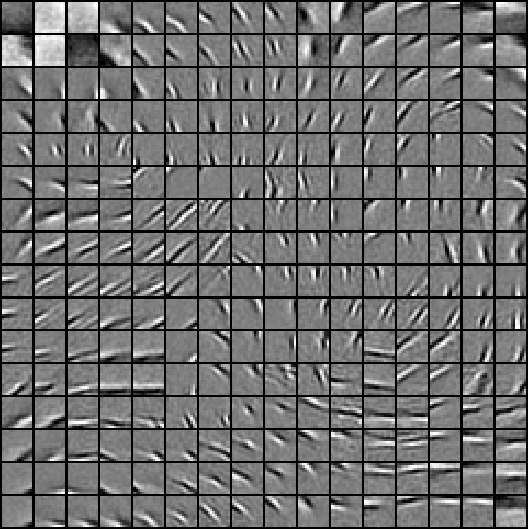
\includegraphics[width=0.4\textwidth]{figures/TopographicSparseCodingFeatures.png}
  %\caption{}\label{fig:step1}
\end{figure}




